\subsection{Implementation}
The kernel trick is a way to add nonlinearity to the SVM model. This can be done efficiently with the kernel trick. We have already seen that we can make the decision boundry of a perceptron non linear by using a feature transform $\Phi: \mathbb{R}^n \leftarrow \mathbb{R}^m$. We have seen in the task before thatthe objective function of the quadratic program contains $ \frac{1}{2} \sum\limits_{i=1}^N \sum\limits_{j=1}^N\alpha_i\alpha_jt_it_j(x_i^tx_j)$. After the feature transform the inner product in this expression would be $\Phi(x_i)^t\Phi(x_j)$. For some feature transforms we can find a kernel $K$ such that $\Phi(x_i)^t\Phi(x_j)=K(x_i,x_j)$. This helps us by not having to calculate the feature transforms and we can use the same formulation and calculations for $\omega_0$ just by replacing the inner product with the Kernel. It is important to note that, without having a explicit $\Phi$, it doesn't make sense to calculate $\omega$. Therefor we have to use the discriminant function derived in task 1 by replacing the inner product with the kernel. The calculation of $\omega_0$ changes to 
\[
	\omega_0 = t_{i_{\max}} -  \sum\limits_{i=1}^N\alpha_i t_i K(\bm{x_i},\bm{x_{i_{\max}}}).
\]

We have used a radial basis function kernel of the form $K(x,y) = \exp(-\frac{\lVert x-y \lVert}{2\sigma^2})$. This leads to a high model complexity.

Moreover we have seen that the formulation before has no solution if the dataset is not linearly separable and that the solution tends to overfit if we have too many training examples. This can be solved by introducing slack variables $\xi_i$ for $1 \leq i \leq N$. This variables will let the SVM model to missclassify examples, but only by incuring a additional cost. We use an additional parameter $C$ to control the additional cost for missclassified examples. The primal quadratic formulation of this is:
\begin{align*}
	\min&&  \frac{1}{2}\lVert w \rVert + C \sum\limits_{i=1}^N \xi_i &\\
	\text{s.t.}&& (\omega^tx_i+w_0)t_i &\geq 1 - \xi_i &1 \leq i \leq N
\end{align*}
We can again reformulate this by considering the dual problam. This is given by following quadratic program
\begin{align*}
	\max&& - \frac{1}{2} \sum\limits_{i=1}^N \sum\limits_{j=1}^N&\alpha_i\alpha_jt_it_j(x_i^tx_j) +  \sum\limits_{i=1}^N \alpha_i &\\
	\text{s.t.}&& \sum\limits_{i=1}^N\ \alpha_i t_i &= 0& \\
	&&0\leq\alpha_i&\leq C& 1\leq i \leq N
\end{align*}
We can use most matrices for \texttt{cvxopt} as before, we only need to change $G$ and $h$, but this is very simple, but we have to be more careful at calculating $\omega_0$ and $\omega$ as there are also wrongly classified support vectors. Support vectors that lie inside the margin, or that are even wrongly classified, have $\alpha_i=C$. We pick again the support vector with the largest $\alpha_i$ of all $\alpha_i$ with $0\leq \alpha_i \leq C$, say with $i = i_{\max}$, and then:
\[
	\omega = \sum\limits_{i=1}^N\alpha_i t_i \bm{x_i}
\]
and 
\[
	\omega_0 = t_{i_{\max}}(1- \xi_{i_{\max}}) - \omega^t\bm{x_{i_{\max}}}.
\]
If we use the kernel trick, the same as above holds and
\[
	\omega_0 = t_{i_{\max}}(1- \xi_{i_{\max}}) -  \sum\limits_{i=1}^N\alpha_i t_i K(\bm{x_i},\bm{x_{i_{\max}}}).
\]

All the sums are only taken over the support vectors, as all other $\alpha=0$.

As small values of C allow many or strongly missclassified examples, we see that $C$ is a regularization parameter. This is especially important with rbf-SVM as the model complexity 

\subsection{Results} 
We wish to explore these newly defined concepts. For this, we take the data set of assignment 1. This is generated by taking images of the handwritten digits $0$ and $7$ and using solidity and eccentricity as features. We use $500$ images per class. 

We first show the result of a SVM with radial basis function and slack in figure\ref{task2::example}. We used a $\sigma = 0.5$ and $C=50$. We see that the decision boundary and margin can  describe a very complex manifold.
\begin{figure}
	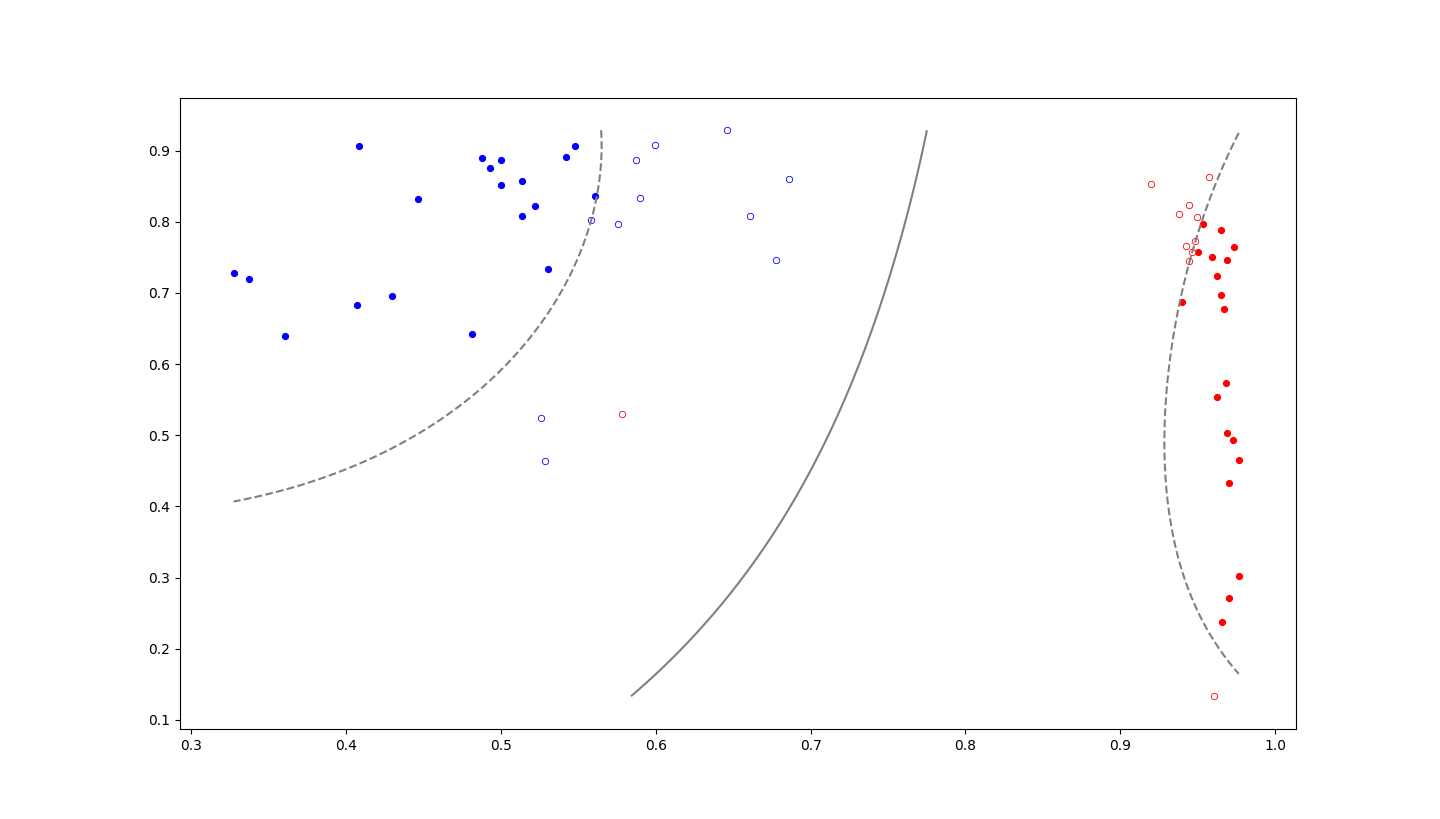
\includegraphics[width = 0.9\textwidth]{new/2_Figure_1}
	\caption{A rbf-SVM with slack. $\sigma = 0.5$ and $C=50$}
	\label{task2::example}
\end{figure}

We also wished to get an overview of what the effect the parameters $C$ and $\sigma$ do. To this end, we trained a rbf-SVM with the same data set and we studied the influence of $\sigma$ and $C$. We used $\sigma\in\left\{ 0.1, 1, 5 \right\}$ and  $C\in\left\{ 1, 10, 100 \right\}$. We show the result in figure \ref{task2::influence}.
\begin{figure}
	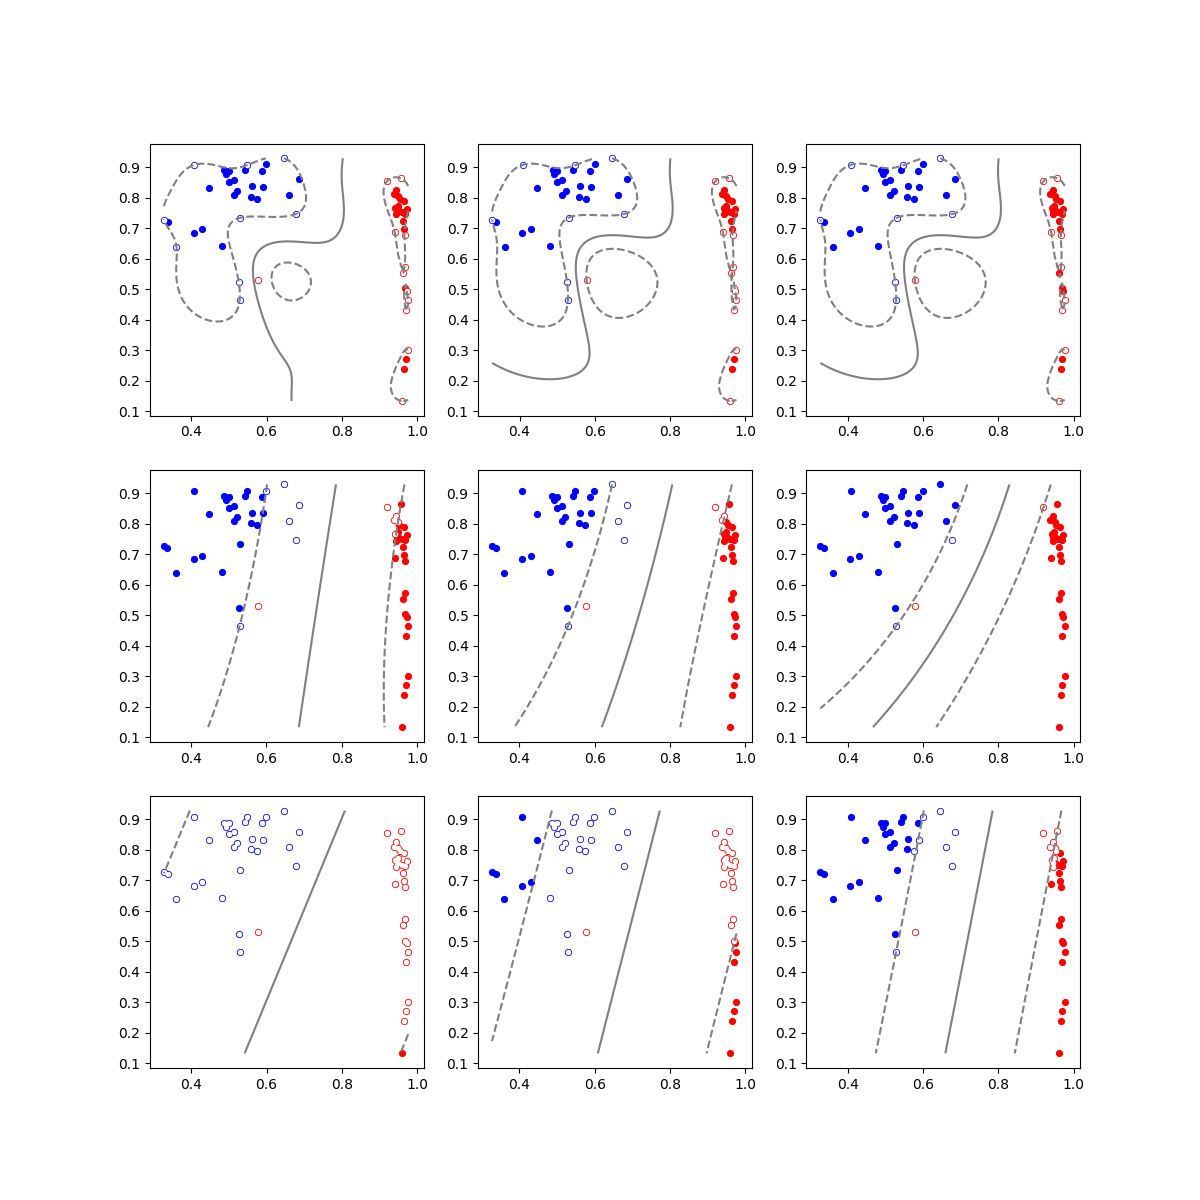
\includegraphics[width = 1\textwidth]{new/2_Figure_2}
	\caption{Slack increases from left to right. $\sigma$ increases from top to bottom}
	\label{task2::influence}
\end{figure}

We see that as slack increases, the solution gets more complicated, or less regular. We can also see that the margin decreases. As $\sigma$ increases, the solution tends to get more linear. This is the case as more and more data points are influencing each other. A smaller sigma has less bias and more variance, and inverse for large sigma.

Following error rates were achieved.
\begin{tabular}{|c|c|c|c|}
\multicolumn{3}{l}{}\\
\multicolumn{3}{l}{Training error}\\
\hline
&1&10&100\\
\hline
0.1&0.023&0.023&0.023\\
\hline
1&0.024&0.023&0.023\\
\hline
5&0.026&0.026&0.025\\
\hline
\multicolumn{3}{l}{}\\
\multicolumn{3}{l}{Test error}\\
\hline
&1&10&100\\
\hline
0.1&0.02959184&0.03010204&0.03163265\\
\hline
1&0.03010204&0.03010204&0.03010204\\
\hline
5&0.03214286&0.03061224&0.03061224\\
\hline
\end{tabular}\\

We repeated the experiment with only 30 instead of 500 data points per class in the training set.

\begin{tabular}{|c|c|c|c|}
\multicolumn{3}{l}{}\\
\multicolumn{3}{l}{Training error}\\
\hline
&1&10&100\\
\hline
0.1&0&0&0\\
\hline
1&0.016667&0.016667&0.016667\\
\hline
5&0.016667&0.016667&0.016667\\
\hline
\multicolumn{3}{l}{}\\
\multicolumn{3}{l}{Test error}\\
\hline
&1&10&100\\
\hline
0.1&0.04744898&0.05867347&0.05867347\\
\hline
1&0.03112245&0.03112245&0.03367347\\
\hline
5&0.03520408&0.03367347&0.03112245\\
\hline
\end{tabular}\\

We see that the model overfits for small $\sigma$, but a low value of $C$ counteracts that.